\subsection{Hidden Markov Models}
\label{sec:hmmExperiments-sachin}

Having examined briefly the theory behind Hidden Markov Models, let us now look at how the training was done offline, and analyse some results from subsequent tests. As mentioned earlier, the apnoeatic states are modelled as the hidden states $\{x_t\}_1^T$, and are elements of the binary set $\{0, 1\}$. The observed signal is annotated every K samples (every minute in the case of the PhysioNet data), so we stack all K samples into $\vec y_t \in \mathbb{R}^d$, ($d = K$). Using the packages \verb!pmtk3! and \verb!HMM Toolbox!, the algorithms were implemented in \verb!MATLAB!\textsuperscript{\textregistered}, along with the conditioning of the data using spectrogram and PCA analysis. Again, \verb!MATLAB!\textsuperscript{\textregistered} is used for convenience and the code can be easily converted to \verb!Java! after experimentation and analysis.

The code used for the training and testing of the data can be found in Appendix \ref{ch:HMMCode} for ease of explanation. Firstly, we examine the mnain script, covering the reading and conditioning of data, spectrogram transformation and PCA analysis. After explaining the various functions created and used in the script till then, we move on to cover the training and testing of the data.

From the code found in the Appendix \ref{sec:apneaHMM}, the \verb!trainIndex! and \verb!testIndex! vectors are used simply for selecting the files to be used, out of 35, for training and the remainder (or less) for testing the accuracy of the diagnosis. Having chosen the files, the next step is to extract and read the files. This is done using the \verb!readData! function, presented in Appendix \ref{ch:readingDataCode}.

The function reads data from the indices specified in \verb!fileIndex! (which is trainIndex in the main script above), and returns O, containing all the observations merged together in a TxD matrix. T is the total number of minutes of data, and D is the number of samples in a minute (6000 in this case), such that there are T annotations in total. The function also returns the vector q, a Tx1 vector containing the latent states for every minute in O, as well as consolidated time, signal and annotation time vectors for ease of plotting and analysis later on.

Firstly, \verb!readData! uses a simple function \verb!getFilenames! to return a 35x1 cell of the available filenames, in a cell string. Then, after initialising the variables, \verb!readData! uses a for-loop to run through each file and extract the relevant information. Using the pre-provided \verb!rdsamp! and \verb!rdann! functions, the signal values as well as annotations are read from the file. As the annotations use `A' for apnoeatic episodes and `N' for non-apnoeatic episodes, the vector type is converted to the alphabet ${0,1}$. The \verb!O! and \verb!q! output matrices are built up using the information from each file, and finally some trivial conditioning is done to ensure ease of plotting if the signal were to be kept.

Armed with the consolidated vectors \verb!X! and \verb!Y!, we now proceed to use the \verb!spectrogram! function in \verb!MATLAB!\textsuperscript{\textregistered}, as described in section~\ref{sec:conditioningExperiments-ta}. We then use the \verb!pca! function from the \verb!pmtk3! package to perform Principal Components Analysis (choosing the number of principal components we wish to include, \verb!k!). 

We then move on to training and fitting the parameters, using the \verb!pmtk3! and \verb!HMM Toolbox! packages. We then compare the expected hidden states calculated using the \verb!Viterbi Algorithm! with the actual underlying states and determine the accuracy of the HMM model diagnosis.

The parameters are fitted using the \verb!apneaHMMTrain! function shown in Appendix \ref{sec:apneaHMMTrain}, which computes the transitional matrix \verb!A! using

\begin{align}
		A_{ij} & = \frac{\sum_{t = 1}^{T - 1} 1\{x_t = s_i \land x_{t + 1} = s_j\}}{\sum_{t = 1}^{T} 1\{x_t = s_i\}}
\end{align}

and uses Gaussian fitting to calculate the pdfs for the emissions (the \verb!gaussFit! function is used from the \verb!HMM Toolbox! package -- we shall not go into the details on how the function is implemented here). We are left with the outputs \verb!A!, the 2x2 transition matrix, \verb!Mu! and \verb!U!, parameters of the Gaussian pdf fit of the emissions, and \verb!pi!, the initial state distribution.

In order to compare with the test data, we need to read the data specified using \verb!testIndex!, condition it, and use the \verb!Viterbi Algorithm! to calculate the most likely path. This is done in the function \verb!apneaHMMTest!, found in Appendix \ref{sec:apneaHMMTest}. The code for reading and conditioning the data (and plotting the results) has been ommitted as it is similar to that shown before. Once again, functions from `off-the-shelf' packages are used in implementing the \verb!Viterbi Algorithm! and the accuracy of the most likely path is calculated by comparing it to the annotations reflecting the true states. This is done for each test file, and the results are shown below.

The results for the HMM experiment are shown in Figure \ref{fig:hmmExperiment}. While the average accuracy is much lower than that found for the SVM model, at 64.1\%, we feel that the HMM model would still be more appropriate than the SVM one due to the absence of Support Vectors which tend to lead to poor generalisation performance. Due to limited computational power and memory (fitting the parameters takes a considerable amount of time on a standard laptop), we were unable to utilise the full set of data for our experiments. However, we are confident that if more time and effort were to be expended in this area, the HMM model would prove to be more accurate in diagnosing apnoea as compared to the SVM model. This is because of the suitability of the Hidden Markov Model for temporal data and the applicability of the Markov assumptions in our case.

\begin{figure}[ht]
		\centering
		\subfloat[record 11]{%
			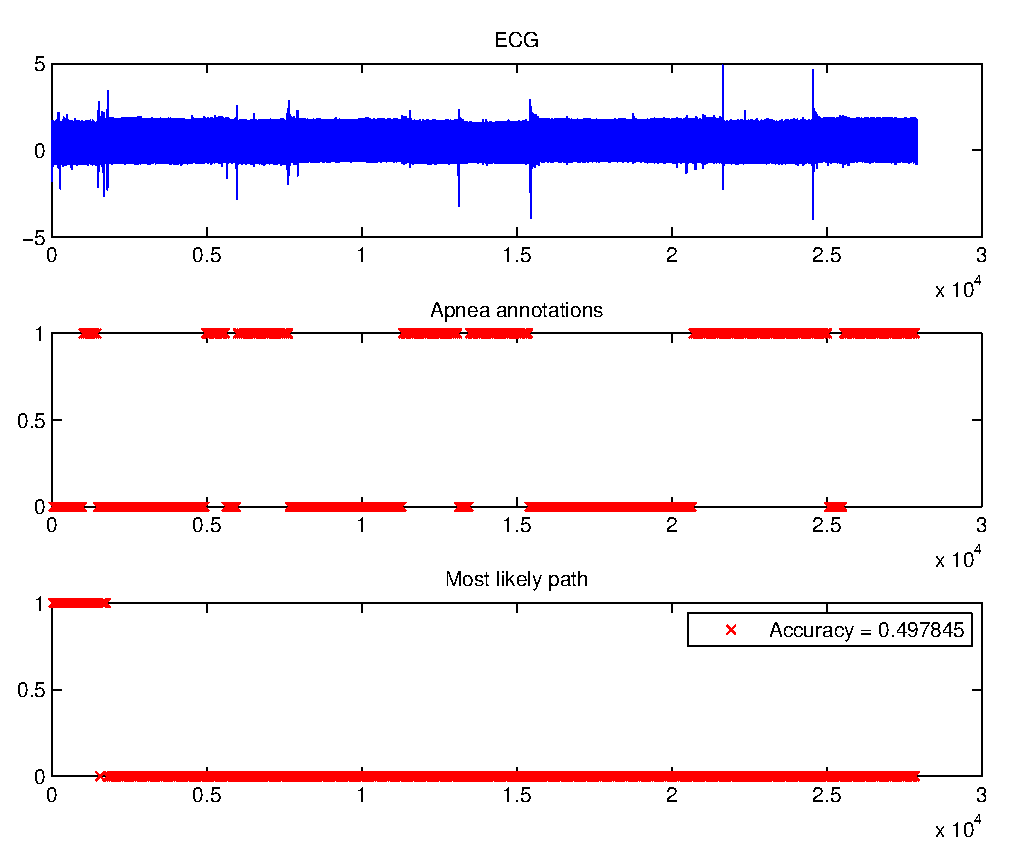
\includegraphics[width=.33\textwidth]{drawings/hmm/hmmTest11}}
		\subfloat[record 12]{%
			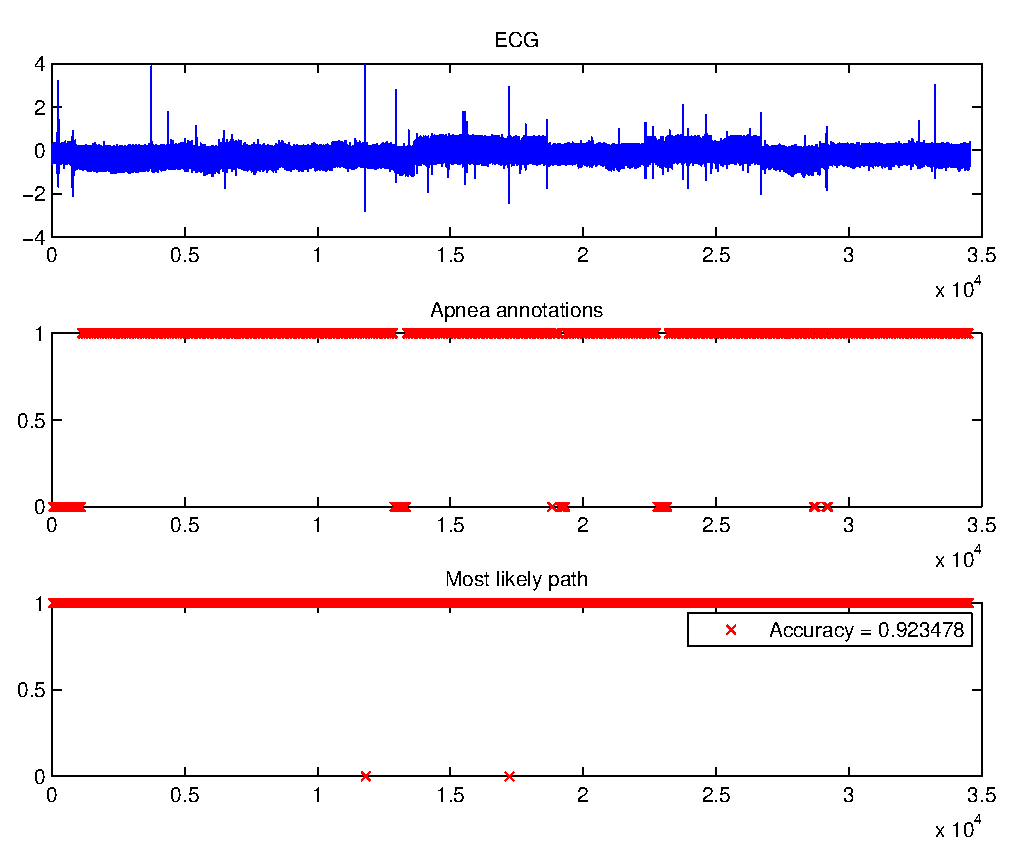
\includegraphics[width=.33\textwidth]{drawings/hmm/hmmTest12}}
		\subfloat[record 13]{%
			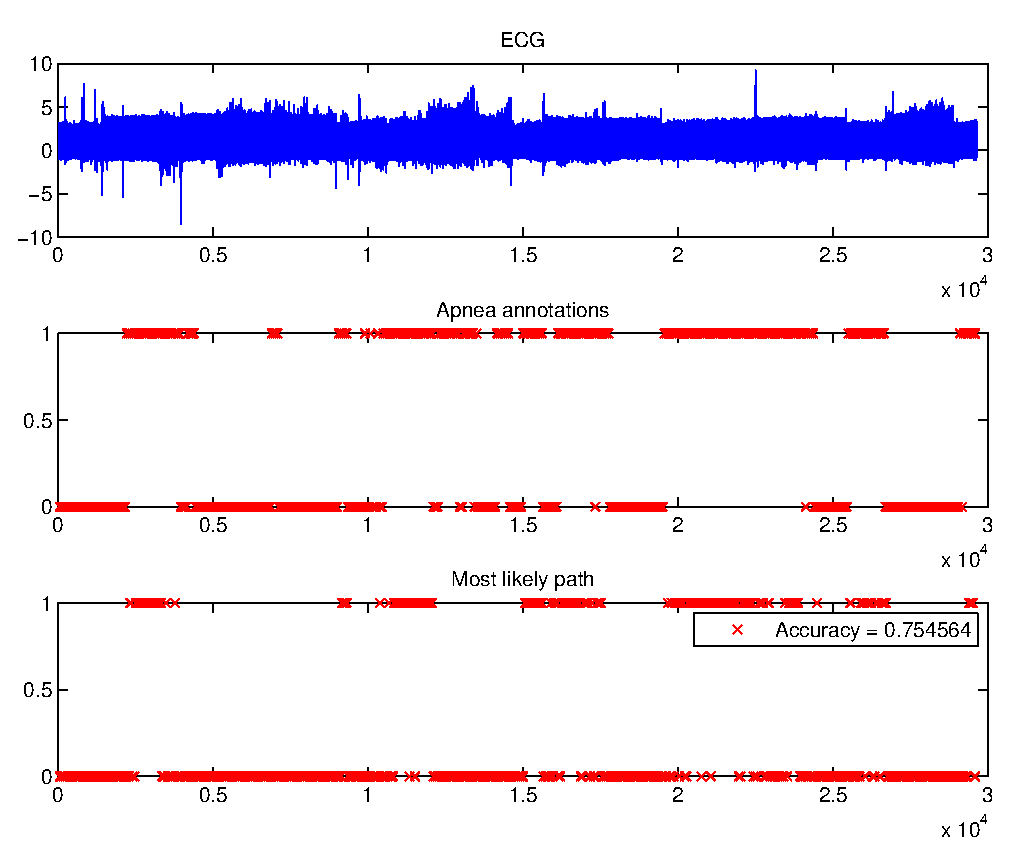
\includegraphics[width=.33\textwidth]{drawings/hmm/hmmTest13}} \\
		\subfloat[record 14]{%
			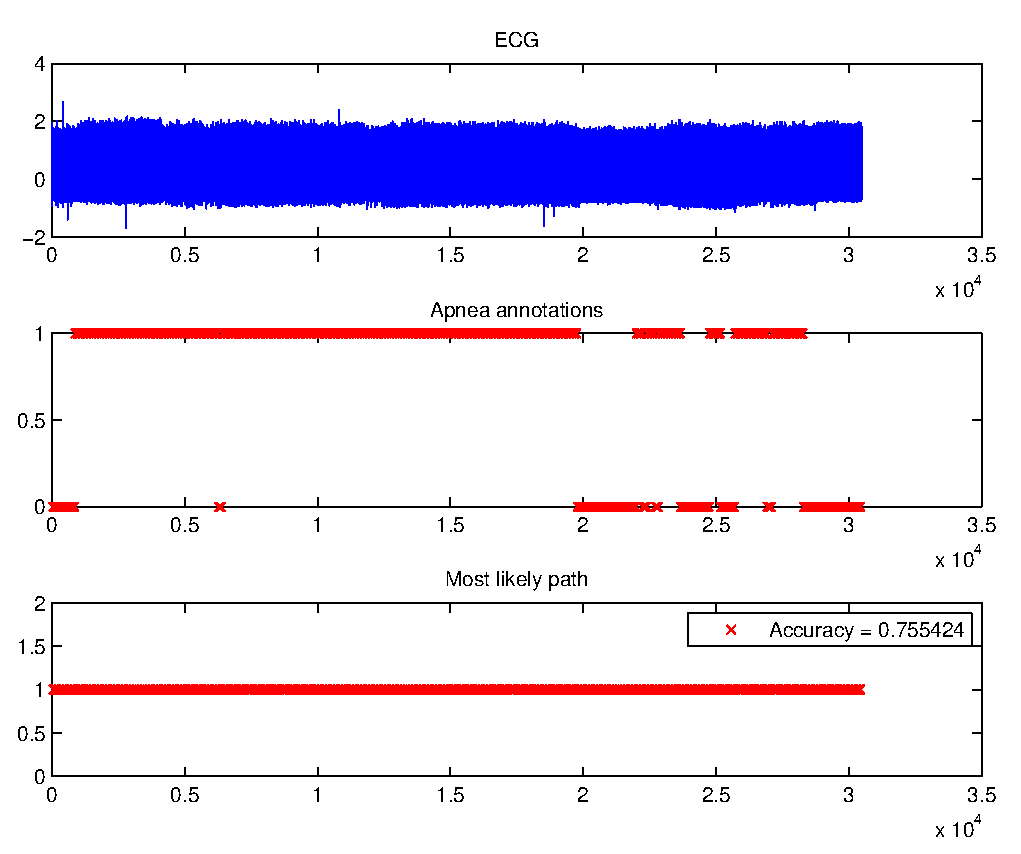
\includegraphics[width=.33\textwidth]{drawings/hmm/hmmTest14}}
		\subfloat[record 15]{%
			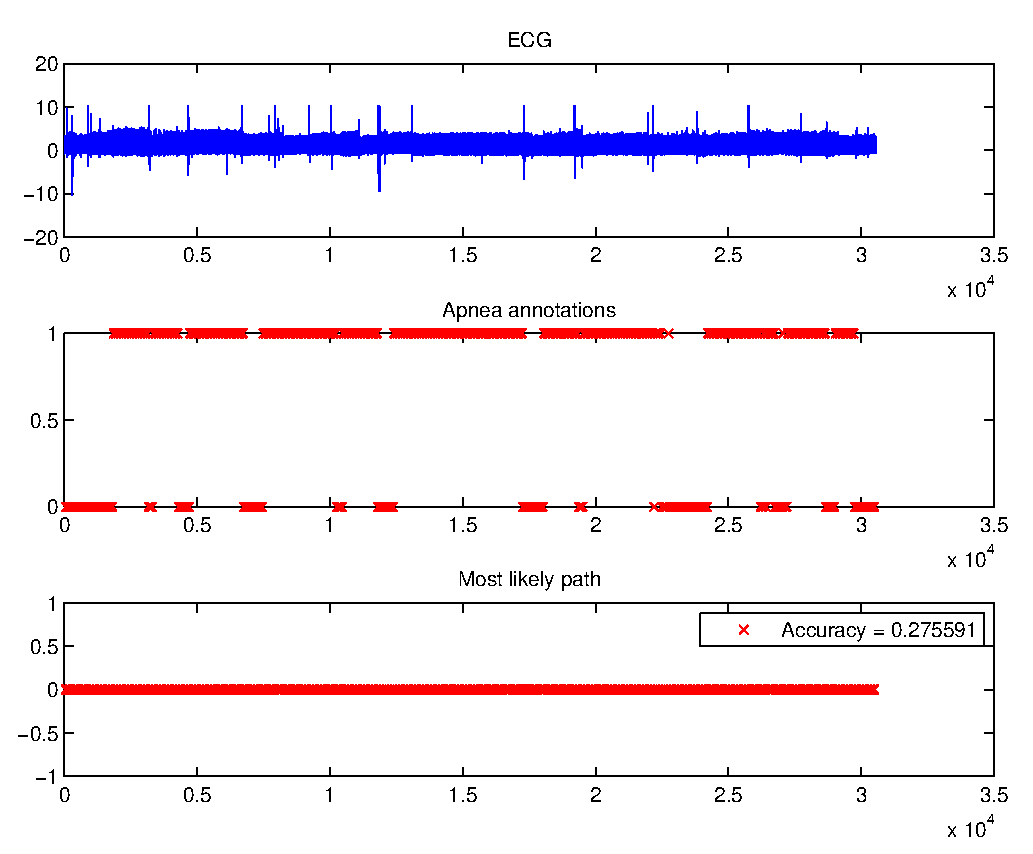
\includegraphics[width=.33\textwidth]{drawings/hmm/hmmTest15}}
		\caption{Performance of HMM model on the test records 11 to 15}
		\label{fig:hmmExperiment}
\end{figure}
